\chapter{Overview}
\label{Overview}

Within the literature discussed, the approaches taken to sentiment analysis are varied. Each proposes its own unique takes on structure, components and design patterns. This project hopes to both utilise and draw together the more successful methods taken when analysing sentiment. Furthermore, in combining them we hope to discover potential improvements and avenues for further exploration. Lastly the project hopes to look at potential methods for further expanding sentiment analysis in order to explore a wider depth and range of emotion.

\section{Design}

The approach we will take within this project can be broadly divided into six core components:

\begin{enumerate}
	\item \emph{Content retrieval} - interfaces with Twitter's various APIs to retrieve relevant twitter statuses for classification. This will serve as the system's main input.
	\item \emph{Subjectivity classification} - given a twitter status, this module will serve as a mechanism for identifying whether the status is opinionated or not.
	\item \emph{Polarity classification} - given an opinionated status, this module hopes to classify it's polarity, along with the strength of the opinion expressed.
	\item \emph{Topic extraction} - given an opinionated status, this module will determine the topics at which the opinion is directed.
	\item \emph{Emotion classification} - given an opinionated status, this module hopes to determine the emotional state of the tweet; classified according to the labels put forward by Plutchik.
	\item \emph{Classification storage} - once classified, statuses must be persisted for use within external modules, such as the visualisation engine.
\end{enumerate}

The way in which these components interlink is best demonstrated visually, as shown in figure \ref{fig:outline_diagram}.

\begin{figure}[h!]
	\caption{Structure for sentiment analysis engine}
	\label{fig:outline_diagram}
	\centering
		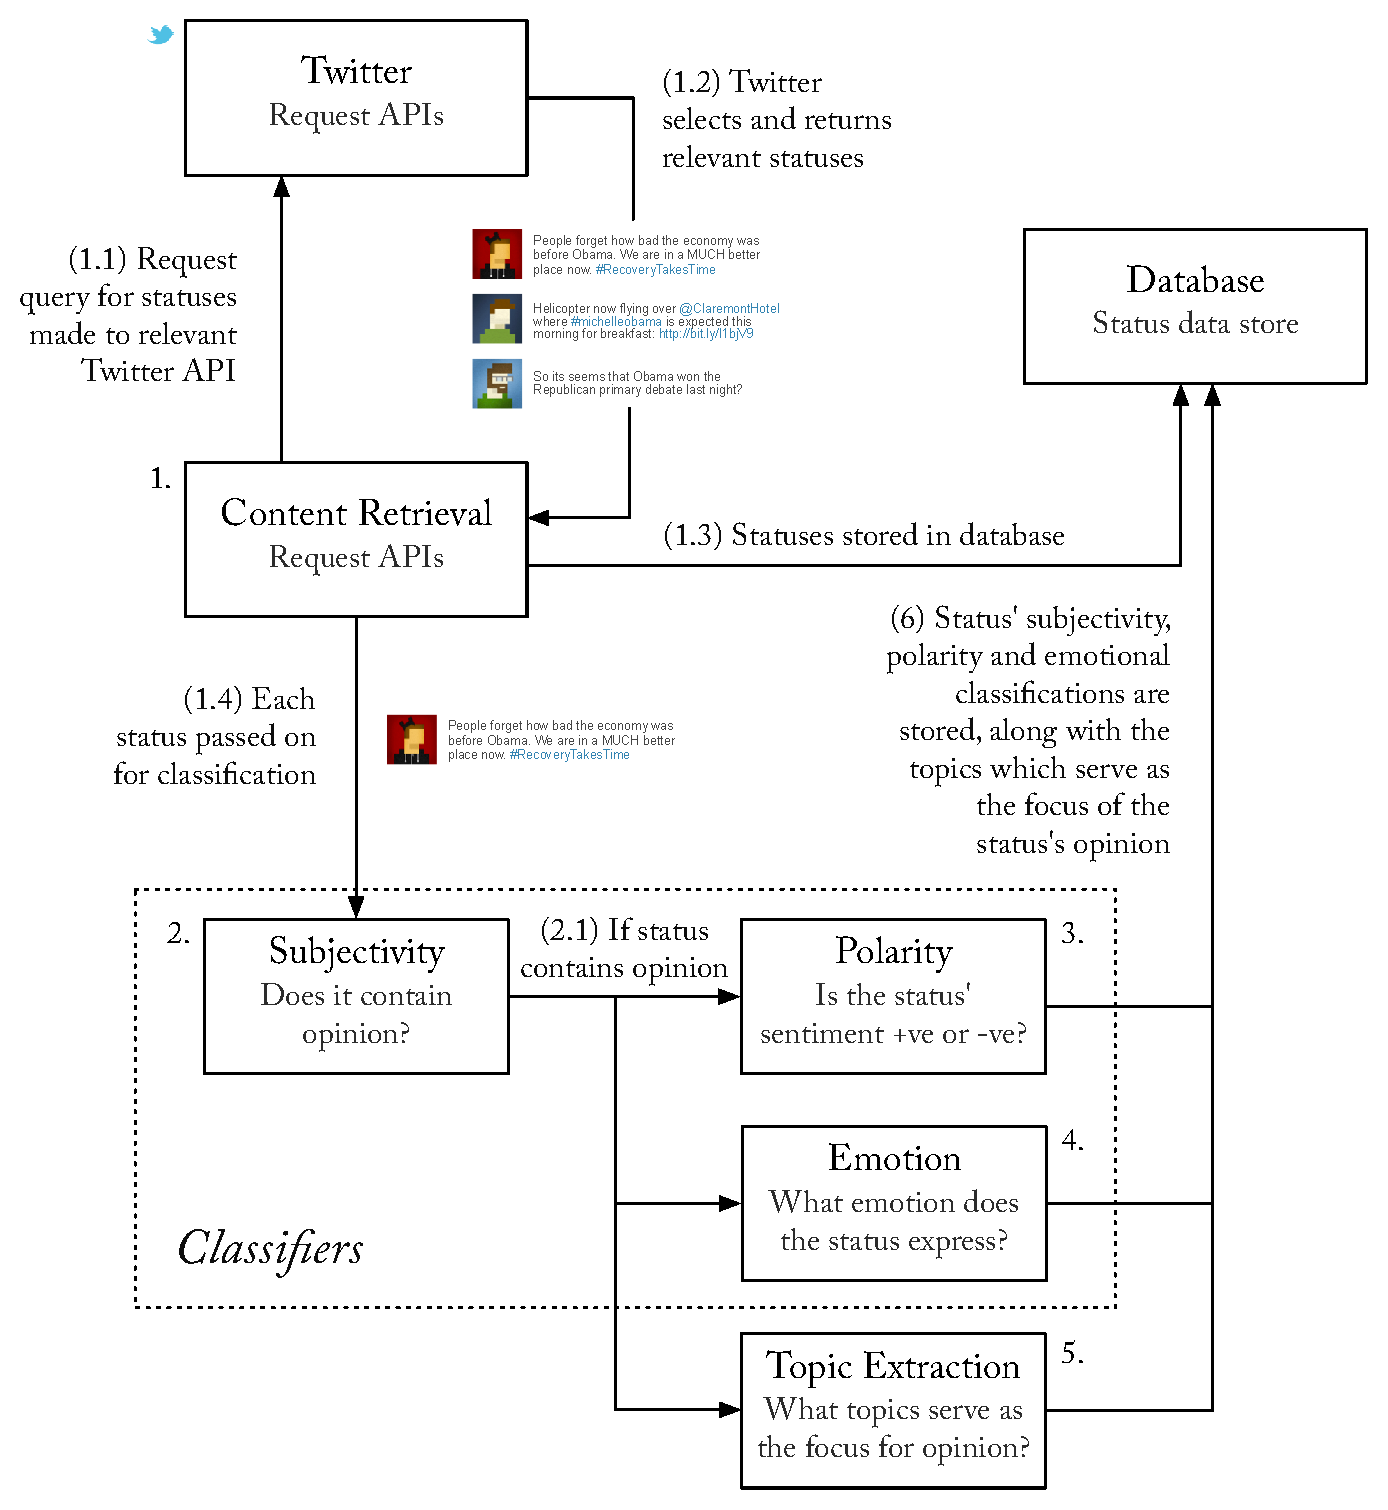
\includegraphics[width=1\textwidth]{figures/outline.eps}
\end{figure}

We will discuss the first five components in more detail in their own relevant chapters. Classification storage will be referenced where relevant in other chapters, however it does not warrant detailed discussion on its own. 

\section{Implementation narrative}

Throughout our discussion of the project's implementation we shall use five example tweets to help illustrate the classification process within the system. 

\begin{tabular}{ | l | p{4in} | }
	\hline
	No. & Text \\
	\hline
	1. & I think David Cameron is doing a rather good job: strong leader, holding together seemingly impossible coalition, keeping labour at bay \\ %(4dfba78ea590e5055600074f)
	2. & BBC Obama, Merkel warn on Europe debt http://bbc.in/jfZW3I \\ %(4dee52e297dee90936000312)
	3. & \#Obama says European debt crisis can't be allowed to threaten global economy. Shame US never felt this way about its financial crisis. \\ %(4dee52e297dee90936000310)
	\hline
\end{tabular}





